\chapter{Modelling Unstructured Text Data}\label{ch:TopicModelling}

\section{Background}

The majority of data currently being produced is unstructured and unclassified.
As a result, there is a need for techniques that automatically organize big,
unclassified corpuses of text. Topic modeling finds clusters of words that
frequently occur together (topics), connects words with similar meanings, and
distinguishes different uses of words with multiple meanings
\cite{alghamdi2015survey}. This is based on the underlying assumption that a
document is generally concerned with a fixed set of topics, and that the
frequency of words used is indicative of this latent structure
\cite{blei2003latent}. Topic modeling has been used extensively to create
recommendation systems, perform trending analysis, and segment text
\cite{alghamdi2015survey}. For the purpose of this research, topic modeling is
necessary to organize the tweets party leaders are promoting by their latent
topics. The ultimate goal of evaluating along what axes the broader populous
engages with political media (policies/topics/issues or party lines)
necessitates a robust way of evaluating messages. To know if people engage based
on various topics requires knowing what those topics are in the first place.
Topic extraction approaches based on keywords are brittle, context specific and
are unable to capture emergent topics. Using unsupervised machine learning
techniques, like the latent Dirichlet allocation discussed in section
\ref{sec:LDA}, topics are able to be extracted in an autonomous manner -
requiring little oversight.

\section{Latent Dirichlet Allocation}\label{sec:LDA}

Blei, Ng and Jordan describe latent Dirichlet allocation (LDA) as a “generative
probabilistic model for collections of discrete data such as text corpora.” The
goal being to extract short descriptions of similar topics from a collection -
and describe statistical relationships that are useful for classification,
summarization, and describing similarity \cite{blei2003latent}. The underlying
thought process behind the LDA is that each document in a corpus can be
described as a distribution of topics, and that each topic can be described as a
distribution of words. 

In this processes, each word in all the text corpus is an element of the
vocabulary, $Voc: \{1,...,V\}$. Each word, $v\in V$, is represented by $w$, a
unit-basis vector of dimension $V$ where:

\begin{numcases}{\text{$w[index=i]$}}
    1   & if $v = i$ \notag \\
    0   & if $v \neq i$ \notag
\end{numcases}

A document is a sequence of $N$ words denoted by $\vect{w} =
(w_{1},w_{2},...,w_{N})$. A corpus is a collection of $M$ documents denoted by
$D = \{\vect{w_{1}},\vect{w_{2}},...,\vect{w_{M}}\}$. 

The input to LDA, $M$, will be the tweets aggregated and cleaned from the tweets
of federal Canadian party leaders described in \ref{sec:motivation}. Aside from
the corpus and $k$ - the number of topics - two other parameters are fed to the
LDA: first, $\alpha$, which is organizes the ground $\theta$ and acts as a
concentration parameter for how documents are modelled as topics. Higher
$\alpha$ values generally implies that documents will be viewed as a mixture of
topics, whereas low $\alpha$ values imply that documents will be viewed as a
belonging to a single topic. Similarly, to model words as topics the parameter
$\eta$ organizes the ground for $\beta$, a Dirichlet distribution. 

The generative model for the LDA uses $\theta$ to choose a topic $z_{n}$ of the
$k$ topics the next word will reside from, and chooses a word $w_{n}$ from
$p(w_{n} |z_{n},\beta$), a multinomial probability conditioned on the topic
$z_{n}$. This processes is described graphically in figure \ref{fig:lda_fiugre}

\begin{singlespacing}
    \begin{figure}[H]
    \centering
    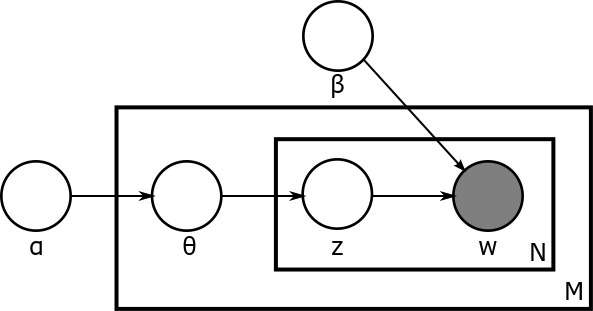
\includegraphics[scale=0.4]{Figures/lda_figure}
    \caption[Graphical Model of the Latent Dirichlet Allocation]{Graphical Model of the Latent Dirichlet Allocation}
    \label{fig:lda_fiugre}
    \end{figure}
\end{singlespacing}

By using variational inference - $\theta$, a distribution of topics for each
document and $\beta$, a distribution of words (one for each topic) can be solved
for giving the final equation
$P(\theta_{1:M},\vect{z}_{1:M},\beta_{1:k}|D,\alpha_{1:M},\eta_{1:k})$
\cite{blei2003latent}.